\chapter{Statistieken}

Via de invoegtoepassing ``Plus for Trello'' is het mogelijk om tal van rapporten te genereren die toelaten om de werking van het project en zijn team te analyseren. We beperken ons in deze handleiding tot de beschrijving van de belangrijkste statistieken.

\section{Overzicht algemene tijdsbesteding}

Dankzij ``Plus for Trello'' is er steeds een algemeen overzicht van de tijdsbesteding te raadplegen in het detailscherm van het Trellobord \korteverwijzing[fig:stats]. In dit overzicht zijn drie verschillende tijdseenheden te zien:
\begin{itemize}
	\item S: Spent, dit de som van uren die de leden gespendeerd hebben op het bord;
	\item E : Estimate, dit is het totaal van alle ingeschatte uren voor de kaarten op het bord;
	\item R : Remaining, verschil van E en S. Dit zijn het aantal resterende uren dat het team nog heeft om aan kaarten op dit bord te werken.
\end{itemize}
Het is mogelijk om deze tijdseenheden te baseren op een andere eenheid dan ``uur'' (bij voorbeeld: minunten of punten). De voorkeur is echter om steeds ``uur'' als tijdseenheid te hanteren.
\begin{figure}
	\centering
	
\includegraphics[scale=0.75]{./afbeeldingen/stats.png}
	\caption{Overzicht tijdsbesteding}
	\label{fig:stats}	
\end{figure} 

\section{Overzicht invididuele tijdsbesteding}

Om de S, E en R uren meer in detail te kunnen anyseren is er de mogelijkheid om een lijst te raadplegen \korteverwijzing[fig:individueleprestatiesknop]. 
\begin{figure}[H]
	\centering
	
\includegraphics[scale=0.75]{./afbeeldingen/individueleprestatiesknop.png}
	\caption{Genereren lijst individuele prestaties}
	\label{fig:individueleprestatiesknop}	
\end{figure} 
\noindent
Hier vinden we een overzicht van alle geleverde (= geregistreerde) prestaties op dit bord opgedeeld per kaart. In dit overzicht \korteverwijzing[fig:individueleprestaties] en op tabblad ``report'' is de lijst opgedeeld in een aantal kolommen. Een overzicht van de belangrijkste kolommen:
\begin{itemize}[nolistsep]
	\item Date: Datum waarop de prestatie geregistreerd werd (niet noodzakelijk zelfde als prestatiedatum);
	\item Card: De kaart waarvoor de prestatie geleverd werd;
	\item List: De lijst (= status) waarin de kaart zich bevindt;
	\item S: Spent = de totale tijd dat het team gepresteerd heeft voor deze kaart;
	\item E1\textsuperscript{st} : First estimate = dit is het totaal aantal uren, som van indivuele inschattingen, die origineel ingeschat werden voor deze kaart;
	\item E : Estimate = aangepaste schatting als er wijzigingen waren na E1\textsuperscript{st};
	\item R : Remaining = verschil van E en S. Dit zijn het aantal resterende uren dat het team nog heeft om aan deze kaart te werken.
\end{itemize}
\begin{figure}[h]
	\centering
	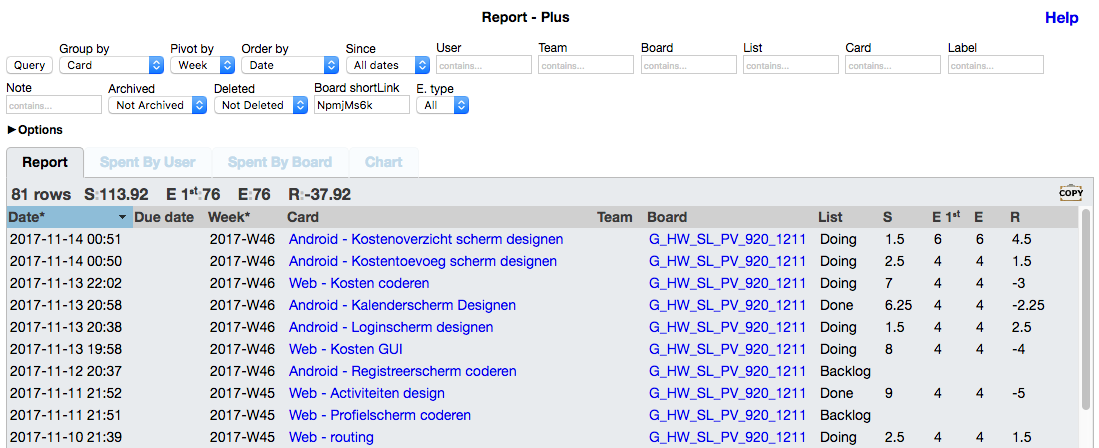
\includegraphics[width=\textwidth]{./afbeeldingen/individueleprestaties.png}
	\caption{Voorbeeld van een lijst met individuele tijdsbesteding}
	\label{fig:individueleprestaties}	
\end{figure} 
Het tabblad ``Spent by user'' geeft je een totaal overzicht van gespendeerde uren per teamlid per week.
Het tabblad ``Spent by board' geeft je een totaal overzicht van gespendeerde uren per bord per week.

\section{Burn-down Chart}

De burn-down chart toont een visueel overzicht van de drie tijdseenheden (S, E en R) voor het huidige bord. Een goede burn-down chart zal er dan ook naar streven om het aantal E uren stabiel te houden gedurende de uitvoering. Deze inschatting begint namelijk bij de aanvang van de iteratie, of aanmaken van het bord, en zou in principe niet meer mogen wijzigen tijdens de uitvoering ervan. Ook worden er normaal gezien geen kaarten toegevoegd tijdens de gesloten iteraties (programmeren). Daarnast zou de burn-down chart dan ook beschikken over een constant dalende curve (R) en een constant stijgende curve (S). Dit zou beteken dat de taken op een evenredig tempo werden afgewerkt waarbij het restrerende aantal uren op het einde van de sprint de 0 benadert.
\\\\
Om de burn-down chart van een bord te kunnen raadplegen gebruiken we de ``report'' knop \korteverwijzing[fig:burndownknop]. 
\begin{figure}[h]
	\centering
	
\includegraphics[scale=0.5]{./afbeeldingen/burndownknop.png}
	\caption{Genereren burn-down chart}
	\label{fig:burndownknop}	
\end{figure} 
\noindent
\\Op het scherm met de effectieve burn-down chart \korteverwijzing[fig:burndownchart] heb je naast de algemene grafiek ook nog de mogelijkheid om deze te verfijnen. Zo kan je de getoonde uren filteren (``View Filter'') of een overzicht raadplegen per gebruiker van zijn S, E en R uren (``View by user''). Daarnaast kan je ook inzoomen op de algemene grafiek door gebruik te maken van het muiswiel.

\begin{figure}[H]
	\centering
	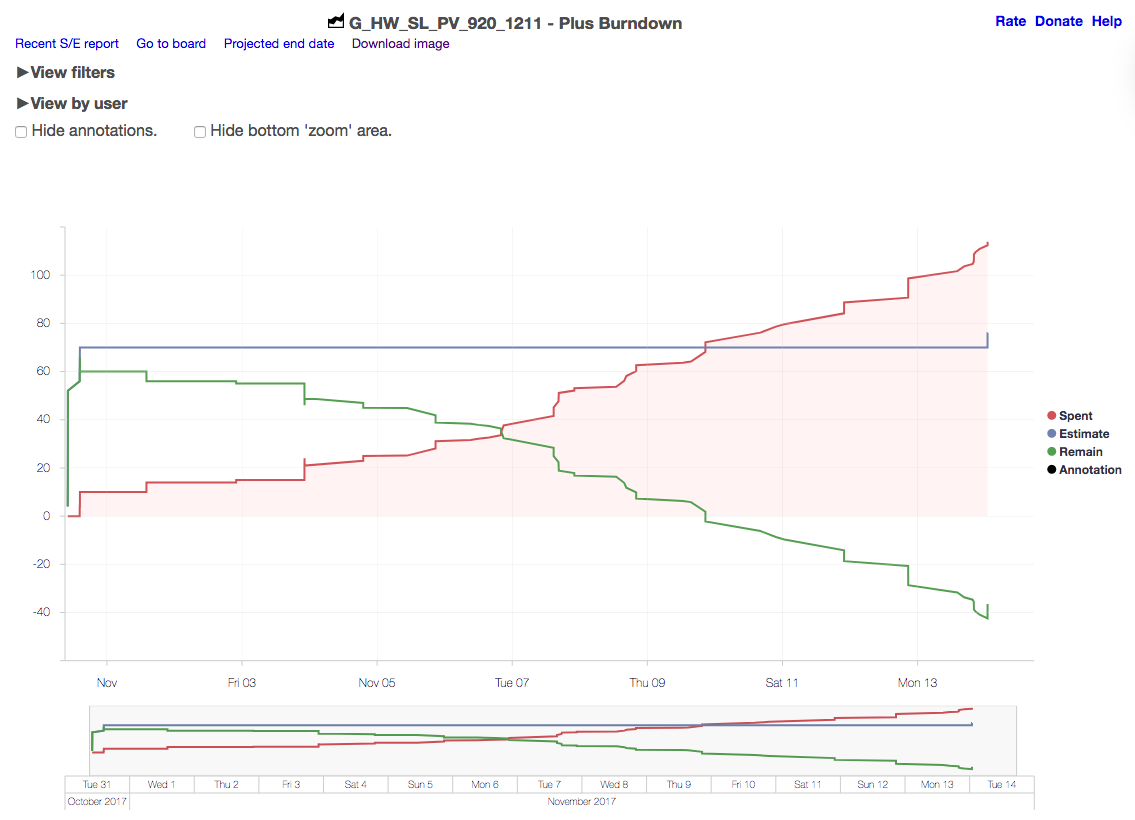
\includegraphics[scale=0.26]{./afbeeldingen/burndownchart.png}
	\caption{Voorbeeld van burn-down chart}
	\label{fig:burndownchart}	
\end{figure} 